Software packaging is the process used to put a software product into an installation package so that it can be installed by the users of the product on their computers. \hypertarget{_software_packaging_SoftwarePackagingOSXPackages}{}\section{O\+S X Packages}\label{_software_packaging_SoftwarePackagingOSXPackages}
In Mac O\+S X world, the installer packages have the file extension .pkg. Instead of distributing multiple files for a package, this allowed all of the software files to be contained in a single file for easier distribution with the benefit of package signing. Package\+Maker is part of the Xcode developer software suite. It provides a comfortable graphical user interface to help users create pkg installer easily. \cite{PackageMaker} 
\begin{DoxyImageNoCaption}
  \mbox{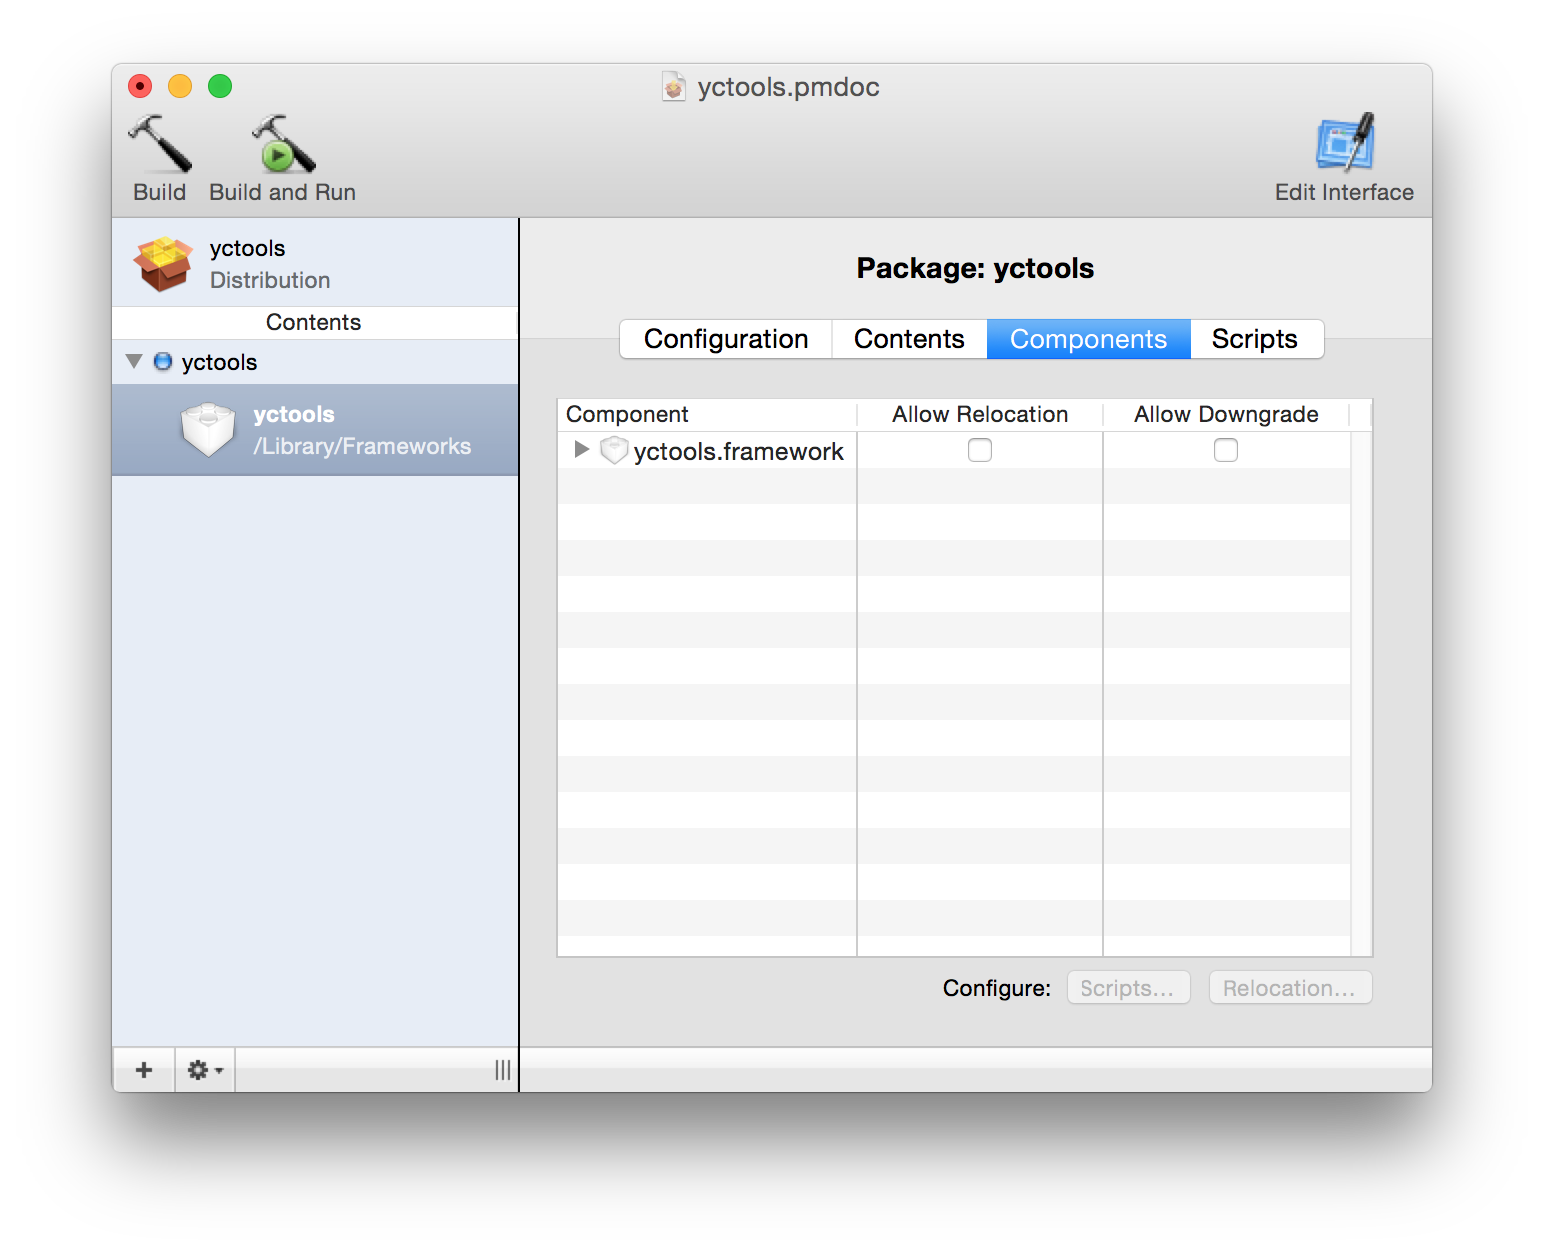
\includegraphics[width=\textwidth,height=\textheight/2,keepaspectratio=true]{ResearchPackegeMaker.png}}
\end{DoxyImageNoCaption}
\hypertarget{_software_packaging_SoftwarePackagingOSXBundle}{}\section{O\+S X Bundle}\label{_software_packaging_SoftwarePackagingOSXBundle}
A Mac O\+S X bundle is a directory that allows related resources such as executable files, graphics, and database to be grouped together, and appears as a single file to the user.
\begin{DoxyItemize}
\item A bundle with extension .app is an application bundle.
\item A framework is an bundle with extension .framework. It contains dynamic library files and header files.
\end{DoxyItemize}\hypertarget{_software_packaging_SoftwarePackagingWindowsInstaller}{}\section{Windows Installer}\label{_software_packaging_SoftwarePackagingWindowsInstaller}
The Windows Installer is a software component used for the software packaging in Windows world. The component contains installation, maintenance, and removal of software. ~\newline
~\newline
Install\+Forge is a free installation creator. It provides a series of functions such as interface design, system environment variable settings, and software update. \cite{installforge} 
\begin{DoxyImageNoCaption}
  \mbox{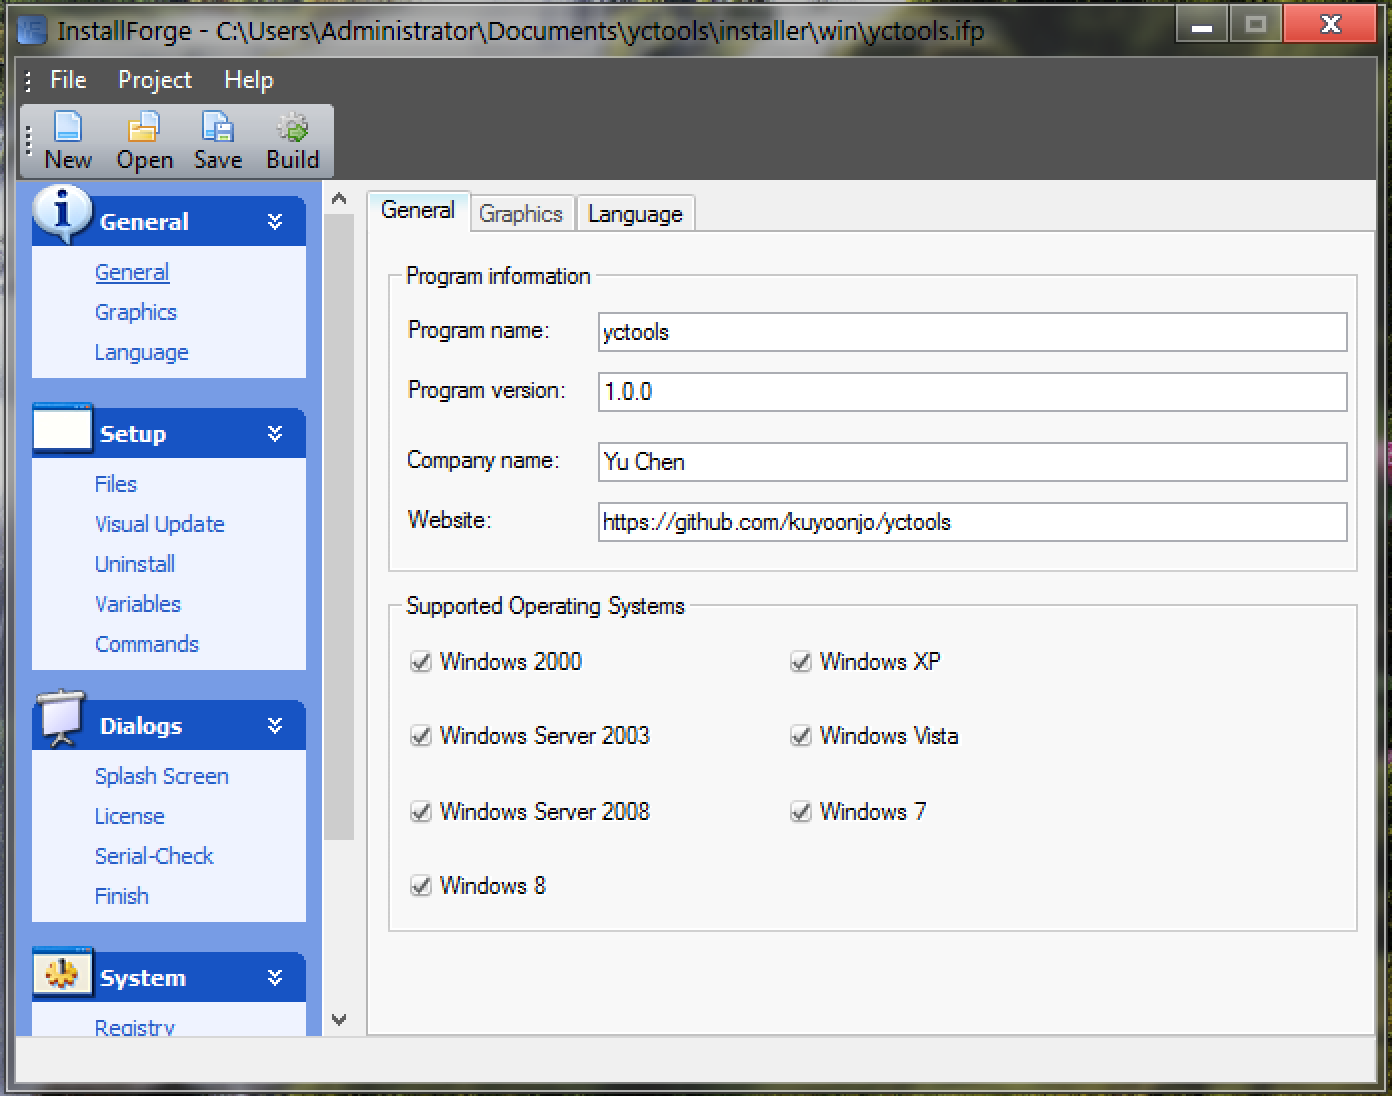
\includegraphics[width=\textwidth,height=\textheight/2,keepaspectratio=true]{ResearchInstallForge.png}}
\end{DoxyImageNoCaption}
\hypertarget{_software_packaging_SoftwarePackagingDebianPackageManagement}{}\section{Debian Package Management}\label{_software_packaging_SoftwarePackagingDebianPackageManagement}
Debian packages generally contain all of the files necessary to implement a set of related commands or features. ~\newline
~\newline
A Debian binary package can contain\+:
\begin{DoxyItemize}
\item executable files
\item configuration files
\item man pages
\item copyright information
\item relative documentation. Linux distributions use Debian package management\+:
\item Ubuntu
\item Debian
\end{DoxyItemize}

Debreate is a Debian package builder. It makes it easy to use graphical user interface for packaging applications. \cite{debreate} 
\begin{DoxyImageNoCaption}
  \mbox{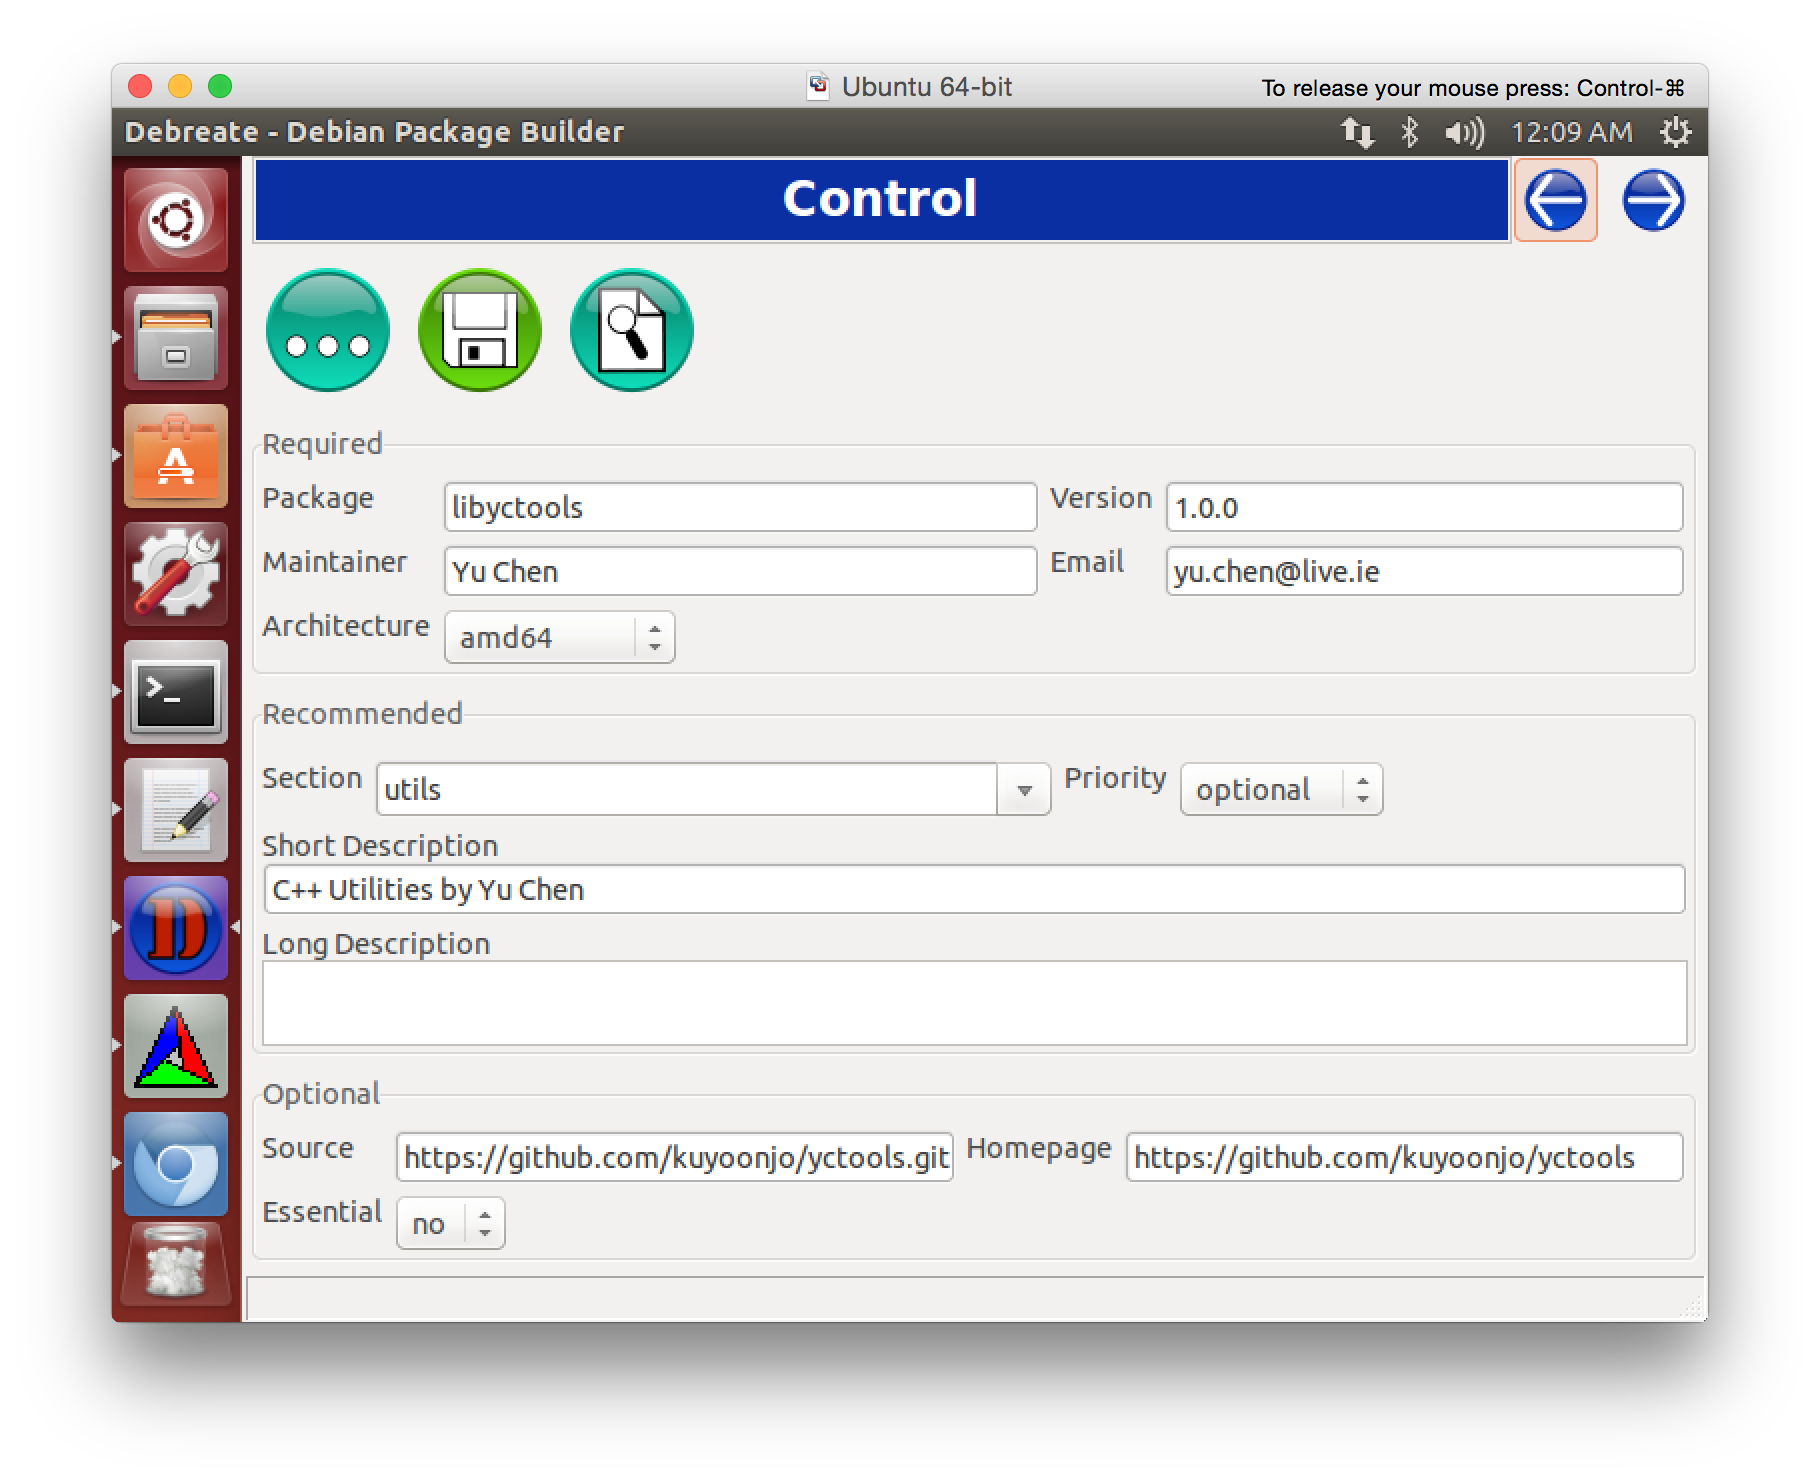
\includegraphics[width=\textwidth,height=\textheight/2,keepaspectratio=true]{ResearchDebreate.png}}
\end{DoxyImageNoCaption}
 